% Created 2023-05-09 Di 20:14
\documentclass{article}

\addtolength{\hoffset}{-2.25cm}
\addtolength{\textwidth}{4.5cm}
\addtolength{\voffset}{-3.25cm}
\addtolength{\textheight}{5cm}
\setlength{\parindent}{0in}
\setlength{\parskip}{5pt}

%-------------------------------------------------------------------------------
%	PACKAGES AND OTHER DOCUMENT CONFIGURATIONS
%-------------------------------------------------------------------------------

\usepackage{charter} % Use the Charter font
\usepackage[utf8]{inputenc} % Use UTF-8 encoding
\usepackage{microtype} % Slightly tweak font spacing for aesthetics
\usepackage[english, ngerman]{babel} % Language hyphenation and typographical rules
\usepackage{amsthm, amsmath, amssymb} % Mathematical typesetting
\usepackage{float} % Improved interface for floating objects
\usepackage{hyperref} % For hyperlinks in the PDF
\usepackage{graphicx, multicol} % Enhanced support for graphics
\usepackage{xcolor} % Driver-independent color extensions
\usepackage{marvosym, wasysym} % More symbols
\usepackage{rotating} % Rotation tools
\usepackage{censor} % Facilities for controlling restricted text
%\usepackage{pseudocode} % Environment for specifying algorithms in a natural way
\usepackage{algorithm}
\usepackage{algorithmic}
\usepackage{booktabs} % Enhances quality of tables
\usepackage{tikz-qtree} % Easy tree drawing tool
\tikzset{every tree node/.style={align=center,anchor=north},
         level distance=2cm} % Configuration for q-trees
\usepackage[backend=biber,style=numeric,
            sorting=nyt]{biblatex} % Complete reimplementation of bibliographic facilities
\usepackage{csquotes} % Context sensitive quotation facilities
\usepackage{fancyhdr} % Headers and footers
\pagestyle{fancy} % All pages have headers and footers
\fancyhead{}\renewcommand{\headrulewidth}{0pt} % Blank out the default header
\fancyfoot[L]{} % Custom footer text
\fancyfoot[C]{} % Custom footer text
\fancyfoot[R]{\thepage} % Custom footer text
\newcommand{\note}[1]{\marginpar{\scriptsize \textcolor{red}{#1}}} % Enables comments in red on margin
\usepackage[utf8]{inputenc}
\usepackage[T1]{fontenc}
\usepackage{graphicx}
\usepackage{longtable}
\usepackage{wrapfig}
\usepackage{rotating}
\usepackage[normalem]{ulem}
\usepackage{amsmath}
\usepackage{amssymb}
\usepackage{capt-of}
\usepackage{hyperref}
\newcommand{\name}{Robert Roth}
\newcommand{\matrikelnr}{1415920}
\newcommand{\email}{s2roroth@uni-trier.de}
\newcommand{\titelname}{Exposé zum Abschlussprojekt}
\newcommand{\vorlesung}{Fortgeschrittene Softwaretechnik}
\author{Robert Roth}
\date{\today}
\title{Expose}
\hypersetup{
 pdfauthor={Robert Roth},
 pdftitle={Expose},
 pdfkeywords={},
 pdfsubject={},
 pdfcreator={Emacs 30.0.50 (Org mode 9.6.5)}, 
 pdflang={German}}
\begin{document}

\fancyhead[C]{}
\hrule \medskip % Upper rule
\begin{minipage}{0.295\textwidth} 
\raggedright
\footnotesize
\name \hfill\\   
\matrikelnr\hfill\\
\href{mailto:\email}{\email} 
\end{minipage}
\begin{minipage}{0.4\textwidth} 
\centering 
\large 
\titelname\\ 
\normalsize 
\vorlesung\\ 
\end{minipage}
\begin{minipage}{0.295\textwidth} 
\raggedleft
\today\hfill\\
\end{minipage}
\medskip\hrule 
\bigskip
\section*{Beschreibung:}
\label{sec:org6aef6d6}
In dem Abschlussprojekt sollen die Themen Continous Integration und Visualisierung in Augmented Reality miteinander vereint werden. Die finale Idee für das Projekt ist aus einer anderen Idee entstanden, die sich so leider nicht umsetzen lässt. Aus diesem Grund werden im Folgenden zwei Ideen vorgestellt.

\emph{1. Idee:}\\[0pt]
In der ersten Idee sollte der Workflow eines Repositories dargestellt werden. Zum Beispiel sollten in GitHub Actions die einzelnen Schritte der .yml-Datei visuell dargestellt werden. Die Visualisierung war dabei wie ein Baum angedacht, in der jeder Schritt ein Knotenpunkt ist und parallele Abläufe werden auf derselben Ebene dargestellt. Das Ganze sollte dann aber 3-Dimensional in Augemented Reality dargestellt werden. Mit anderen Worten: Jeder Knotenpunkt kann als Grundobjekt Sphäre in Unity dargestellt werden. So können die Daten aus GitHub Actions, die Teil des Themenblocks Continous Integration sind, visuell für eine Augmented Reality Anwendung dargestellt werden und so zwei Themen vereinen.\\[0pt]
Wie in Abbildung \ref{fig:orgbd88146} zu sehen, soll erst Task 1 abgeschlossen werden. Danach laufen 2 und 3 parallel. Anschließend laufen 4 und 5 parallel und danach 6 und 7.\\[0pt]
Dabei ergibt sich jedoch ein großes Problem: Die Abläufe sind nicht parallel, sondern meistens in einer klaren Reihenfolge. Dadurch ergibt sich dann keine Baumstruktur, sondern ein Zeitstrahl. Die Visualisierung eines Zeitstrahls ist dann Teil der zweiten Idee geworden.

\begin{figure}[htbp]
\centering
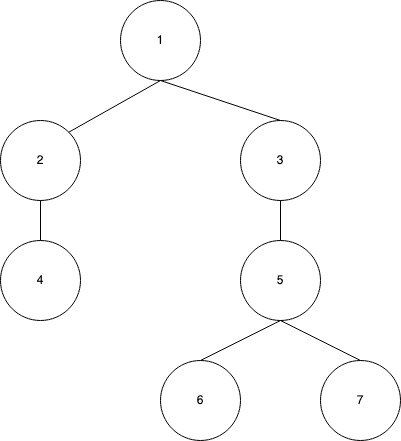
\includegraphics[width=300px]{./img/Idee1.jpg}
\caption{\label{fig:orgbd88146}Beispiel für einen Baum wie in der ersten Idee beschrieben.}
\end{figure}

\emph{2. Idee:}\\[0pt]
Bei diesem Ansatz sollen die Schritte des Workflows ganz bewusst als Zeitstrahl dargestellt werden. Dabei sollen Schritte, die erfolgreich gelaufen sind, als grüne Sphäre dargestellt werden. Wenn ein Schritt fehlschlägt, so wird dies als rote Sphäre dargestellt. Wenn ein Schritt übersprungen wurde, weil beispielsweise ein vorheriger Schritt fehlgeschlagen ist, so soll dies als graue Sphäre dargestellt werden. Wenn man eine Sphäre berührt, so soll ein Tooltip erscheinen, der den Namen des jeweiligen Schritts anzeigt bzw. im Fall eines fehlgeschlagenen Schritts außerdem auch eine Fehlermeldung.\\[0pt]
Auf die Daten kann mithilfe einer REST API von GitHub Actions zugegriffen werden. Mit anderen Worten, man kann auf die Daten jedes öffentlichen Projekts zugreifen und, wenn vorhanden, die Schritte des Workflows abfragen. In der finalen Version soll es möglich sein, ein öffentliches Projekt und die entsprechende Run-ID anzugeben und dann entsprechend den Verlauf des Runs dargestellt zu bekommen.

\largeskip

\begin{figure}[htbp]
\centering

\includegraphics[width=300px]{./img/Idee2.jpg}
\caption{\label{fig:org084e5ca}Zeitstrahl, bei dem die ersten drei Tasks laufen und der vierte fehlschlägt, wodurch die restlichen Tasks übersprungen werden.}
\end{figure}
\end{document}